\begin{figure}[H]
    \centering
    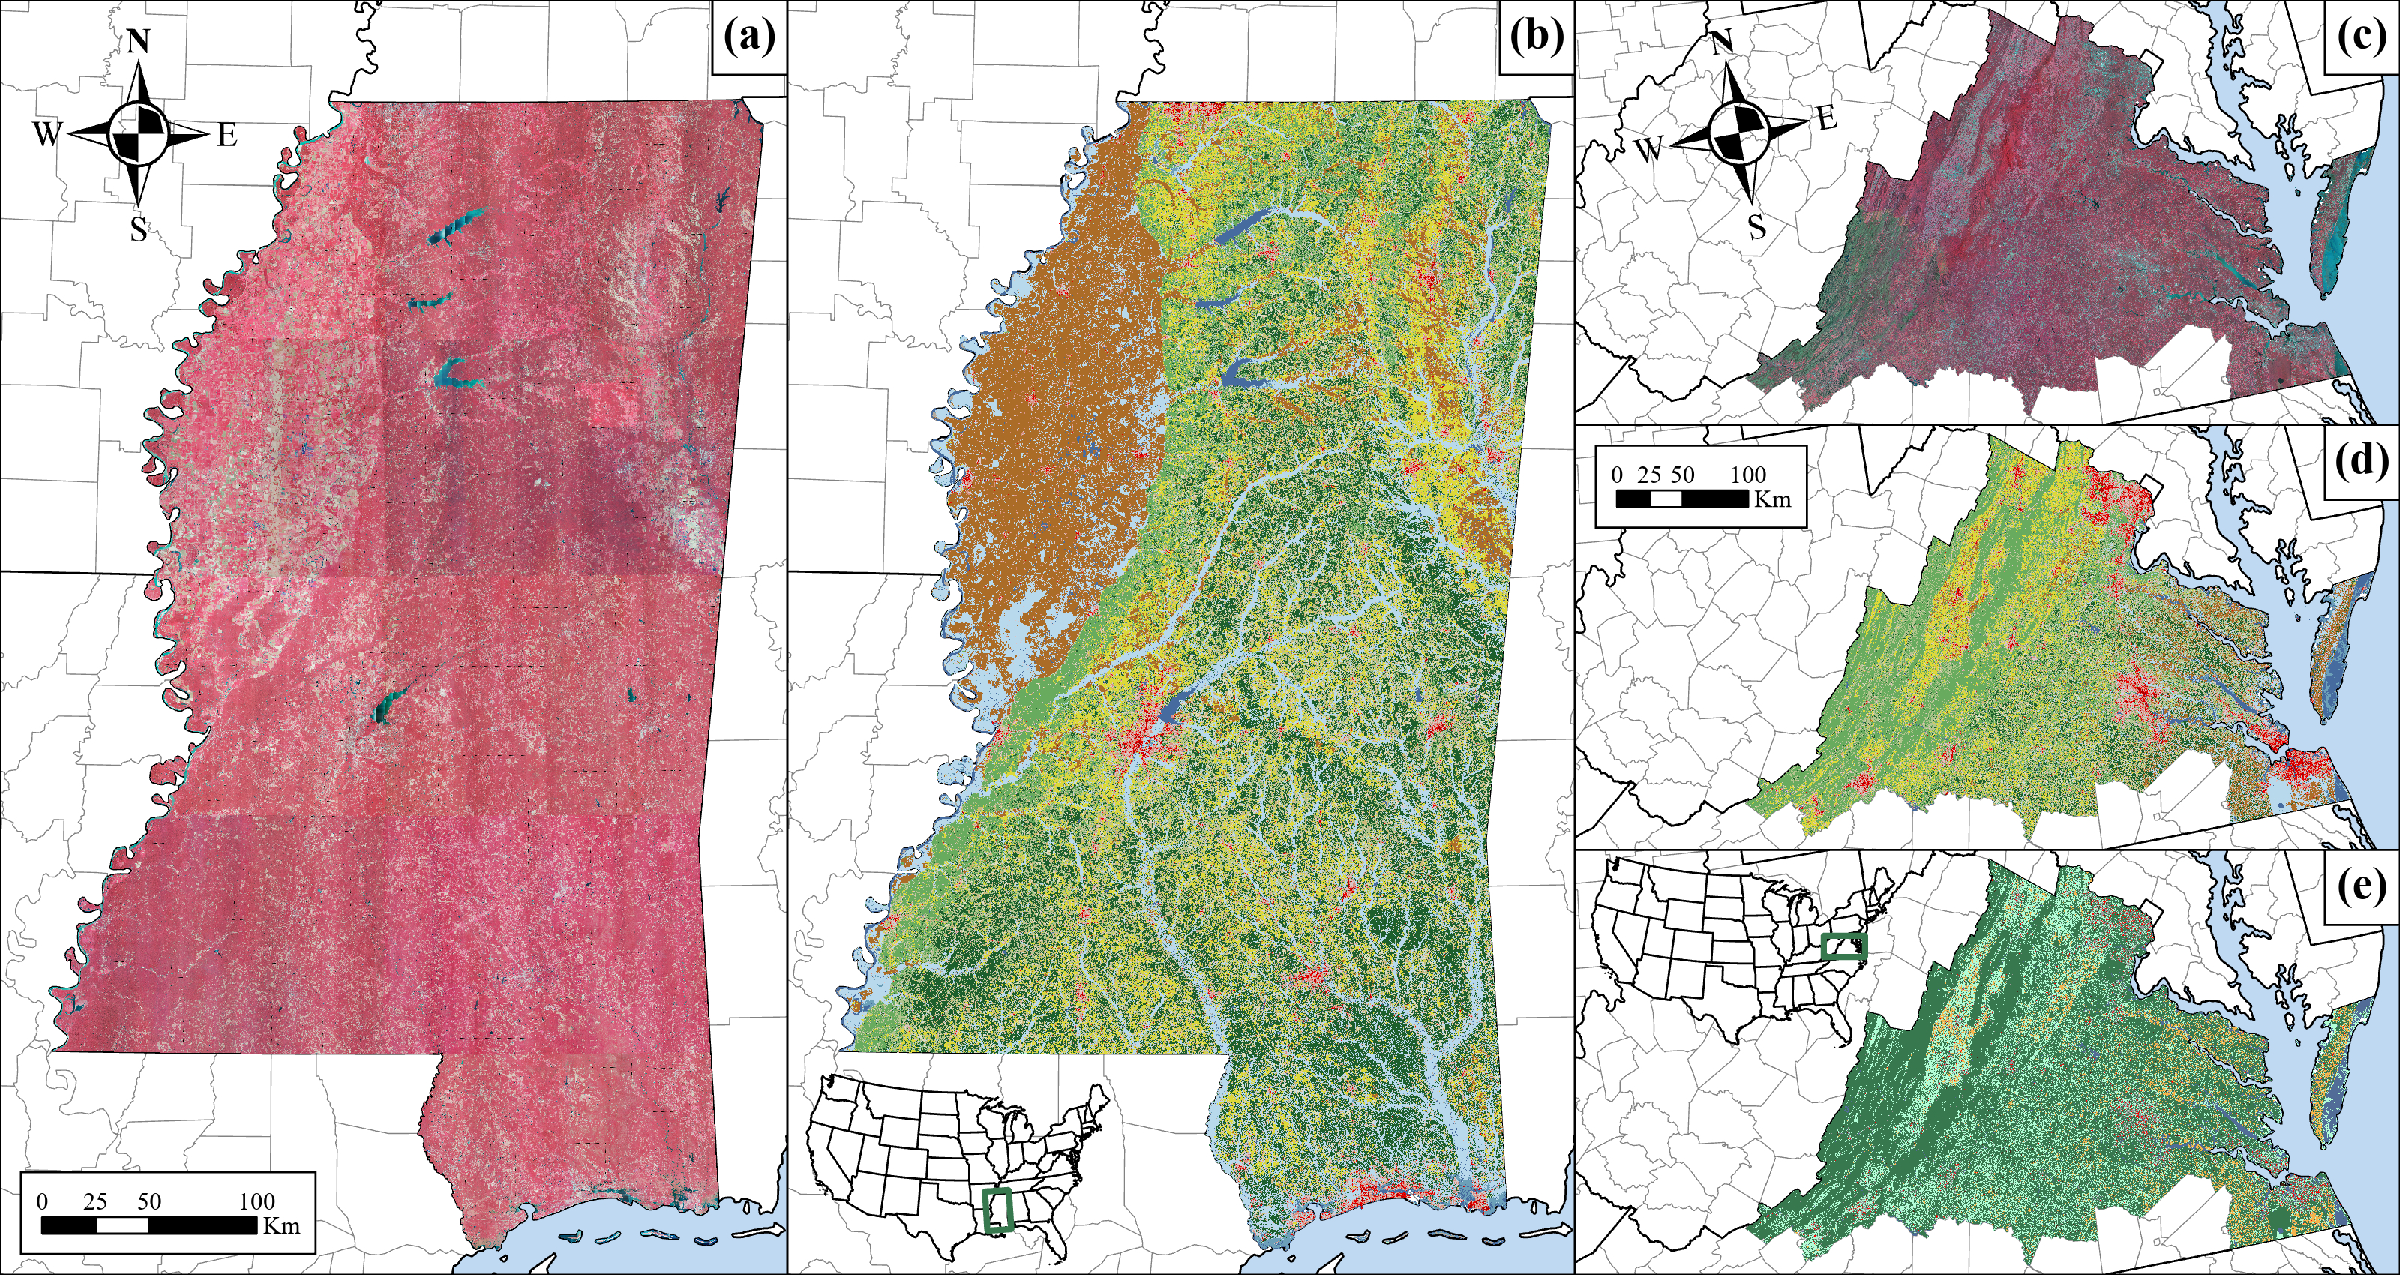
\includegraphics[width=\textwidth]{images/Study_Area.pdf}
    % \caption{Study areas and data sources used in this work: (a) NAIP imagery over the primary study area in Mississippi (b) NLCD 2021 land cover for Mississippi, USA; (c) NAIP imagery over the Chesapeake Bay watershed in Virginia, USA. Imagery over this area will be used to validate a sampling strategy given \SI{1}{\meter} land cover data is pubclicly available for this region; (d) NLCD 2022 land cover map over the Chesapeake Bay watershed in Virginia, USA; (e) CBLC \SI{1}{\meter} land cover map over the Chesapeake Bay watershed in Virginia, USA.}\label{fig:study_areas}
    \caption{The two study areas and corresponding data sources used in this work. (a, b) NAIP imagery and NLCD 2021 land cover for the primary area of interest in Mississippi, USA. (c, d, e) NAIP imagery, NLCD 2022, and \SI{1}{\meter} CBLC data for a subset of the Chesapeake Bay watershed located in Virginia, USA. \note{MOVE VA MAPS SO FULL AOI IS IN FRAME}}\label{fig:study_areas}
    
\end{figure}